%
% File acl2020.tex
%
%% Based on the style files for ACL 2020, which were
%% Based on the style files for ACL 2018, NAACL 2018/19, which were
%% Based on the style files for ACL-2015, with some improvements
%%  taken from the NAACL-2016 style
%% Based on the style files for ACL-2014, which were, in turn,
%% based on ACL-2013, ACL-2012, ACL-2011, ACL-2010, ACL-IJCNLP-2009,
%% EACL-2009, IJCNLP-2008...
%% Based on the style files for EACL 2006 by 
%%e.agirre@ehu.es or Sergi.Balari@uab.es
%% and that of ACL 08 by Joakim Nivre and Noah Smith

\documentclass[11pt,a4paper]{article}
\usepackage[hyperref]{acl2020}
\usepackage{booktabs}
\usepackage{graphicx}
\usepackage{times}
\usepackage{latexsym}
\renewcommand{\UrlFont}{\ttfamily\small}

\usepackage{microtype}

\aclfinalcopy % Uncomment this line for the final submission


\newcommand\BibTeX{B\textsc{ib}\TeX}

\title{Sentiment Analysis for Biochemistry Class Reviews}

\author{Maddie Bonanno \\
  Tulane University / New Orleans, LA \\
  \texttt{mbonanno@tulane.edu} }

\date{}

\begin{document}
\maketitle

\begin{abstract}
Most college STEM courses are lecture style and emphasize memorization over understanding. One Tulane professor runs their classroom in a different manner. To track student opinions, they survey several times a semester. This project investigates the possibility of performing sentiment analysis on these reviews -  can a model predict how a student feels about biochemistry? Survey data was manually labeled and tokenized. It was then fed into a logistic regression, a hidden markov model, and a recurrent neural network respectively. These results indicate there may be valuable information that can be accurately predicted from class reviews.


\end{abstract}



\section{Introduction}




\subsection{Problem Overview}

The goal of this project is to evaluate how an accessible - yet unconventional - teaching style utilized by a Tulane STEM professor has impacted biochemistry comprehension and student enjoyment. Promoting accessibility within the hard sciences can be challenging, but the efforts of one professor go the extra mile. To assess how students feel about these policies, the professor collects survey data regularly. This project will be utilizing sentiment analysis to process all of these responses. The problem is interesting because if things work out, this would be genuinely helpful information for the professor to have. Through this project, I hope to leverage my computer science skills to help someone who has supported me through my academic journey.

\subsection{Data}

The data for this project was collected by the aforementioned professor. Each semester, students are given surveys that question what they’ve learned. By asking for honest written feedback on teaching style and classroom environment, the datasets are full of honest feedback, both negative and positive. 

Due to some factors outside of my control, I was unable to collect all the desired data from the target professor. This forced me to pivot and adjust my strategy. I ultimately decided to form two datasets:
\begin{enumerate}
    \item Small Dataset: composed of 53 sentences [derived from biochemistry class reviews for the aforementioned professor]
    \item Large Dataset: composed of 173 unique sentences. It includes the 53 values from the small dataset plus 120 more sentences collected from Rate My Professor. Given that there was not enough information on just the target professor, the training data was expanded to include reviews for other Tulane professors that teach in the CELL department
\end{enumerate}
Both datasets were composed of similar amounts of positive reviews [sentiment label = 1] and negative reviews [sentiment = 0]


\section{Related Work}

While brainstorming ideas for this project, I found a number of related studies that provided valuable insight.

One key example is the work of \citet{Kastrati_studentfeedback} who explored mechanisms for evaluating student reviews. This study aggregates data from dozens of papers, presenting the most commonly used tools for NLP analysis in this realm. It was found that the most popular tool leveraged for sentiment analysis was the python nltk library \citep{Kastrati_studentfeedback}. Therefore, I began researching this module and the tools I could apply. Sure enough, I ended up using nltk for several components of the project. By looking at how published research papers handled student review processing, I was able to avoid common pitfalls before they occur .

My ultimate goal was to utilize more complicated, pre-trained models. Thus, a lot of my prior research revolved around transformers/highly complex networks. In a study investigating the effectiveness and success of four different sentiment analysis tools, BERT performed the best overall \citep{Alaparthi_bert}. Other works support these findings, emphasizing the success of BERT on both labeled and unlabeled datasets \citep{Chakraborty_unlabeled}. I furthermore looked into pre-trained models that understand scientific jargon, which will likely arise in biochemistry reviews. One fascinating paper from \citet{Susnjak_lyme} describes how BERT can be used to classify perceptions on Lyme disease. Even though my goals weren't necessarily medical in nature, this study provided insight on the capabilities of sentiment analysis at that intersection of scientific topics and opinions. NLP tools  have even been applied in drug development settings \citep{Bhatnagar_drug}, highlighting just how versatile these models can be.

Now, due to the constraints of my dataset, I did not end up using a transformer at all. Instead, my main resource became NLP class notes. I did decide to explore using GloVe embeddings \citep{pennington-etal-2014-glove} within my project as well.


\section{Methods}

Before beginning this project, I was hoping to use a BERT model for my sentiment analysis task. However, I chose to use less complex models that were better suited for my relatively small dataset. My process was the following:


\begin{enumerate}
    \item Firstly, I had to process the raw course reviews. Each document was assigned a sentiment label - 1 represents "positive" while 0 represents "negative"
    \item Each document was then parsed and tokens were generated. This was made possible through the utilization of nltk tools. The tokenization process included
    \begin{itemize}
        \item Removing punctuation and special characters
        \item Converting each word to lowercase
        \item Removing stopwords [such as "me", "the", "and", etc.] 
    \end{itemize}
    \item Then I experimented with several approaches:
    \begin{enumerate}
        \item Building a naive bayes classifier [i.e. I used token frequency to build a simple "Bag of Words" model]
        \item Performing logistic regression on one hot encoded vectors [for both the large dataset and small dataset]
        \item Constructing a basic neural net with one hot encoded vectors
        \item Leveraging GloVe embedding to perform logistic regression
        \item Working with POS tagging for enhanced performance [but accidentally building an HMM model to predict POS for sentences]
        \item Building an RNN and using one-hot encoding vectors
        \item Attempted to construct an RNN using GloVe embedding
    \end{enumerate}
    
\end{enumerate}





\section{Results}

While exploring different models, a number of results were found:

\begin{figure}[h]
    \centering
    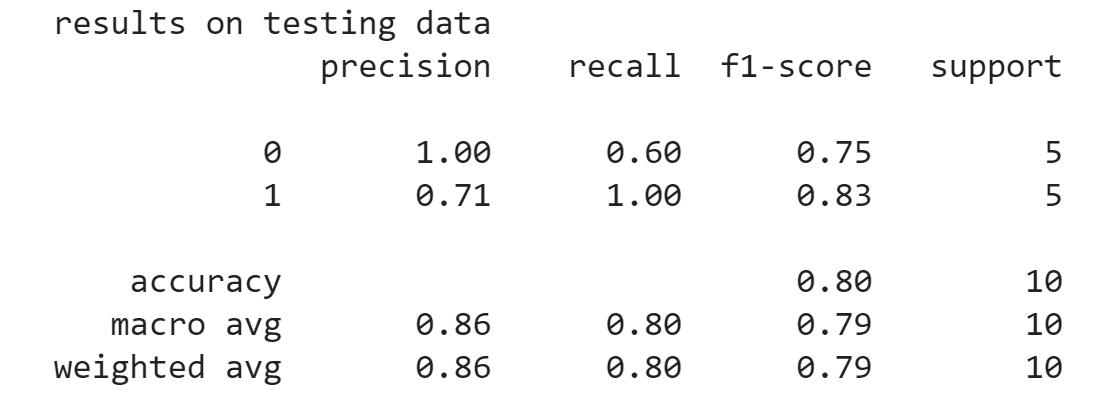
\includegraphics[width=1\linewidth]{NB_result.png}
    \caption{Naive Bayes Classification - Small Dataset}
\end{figure}

Initially, Naive Bayes performed with a decent level of accuracy [close to 0.8]. When run on the larger dataset, this value improved to 0.94.

\begin{figure}[h]
    \centering
    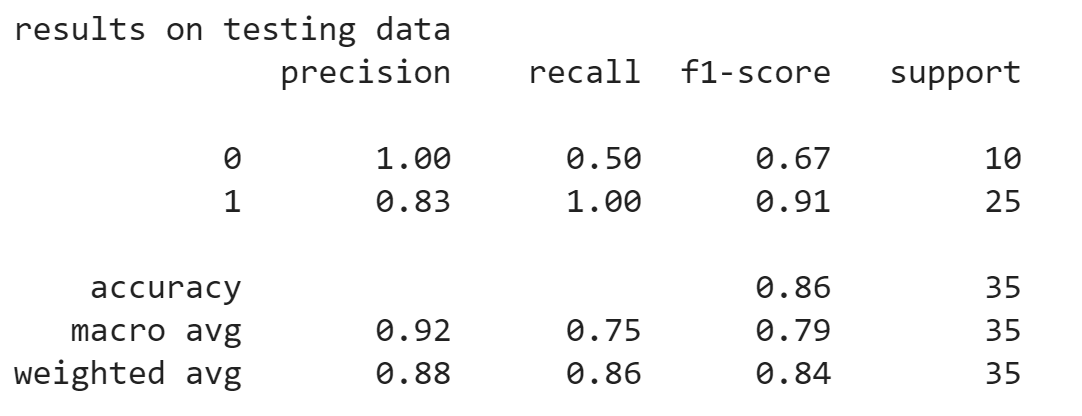
\includegraphics[width=0.75\linewidth]{log_regression_large.png}
    \caption{Logistic Regression - large dataset}
\end{figure}

Running logistic regression on the large dataset was also successful, returning an accuracy of 0.86 [versus a 0.40 for the small set]. This inspired me to continue working with the bigger vocabulary.

When attempting to construct a basic neural net, my attempts fell short

\begin{figure}[h]
    \centering
    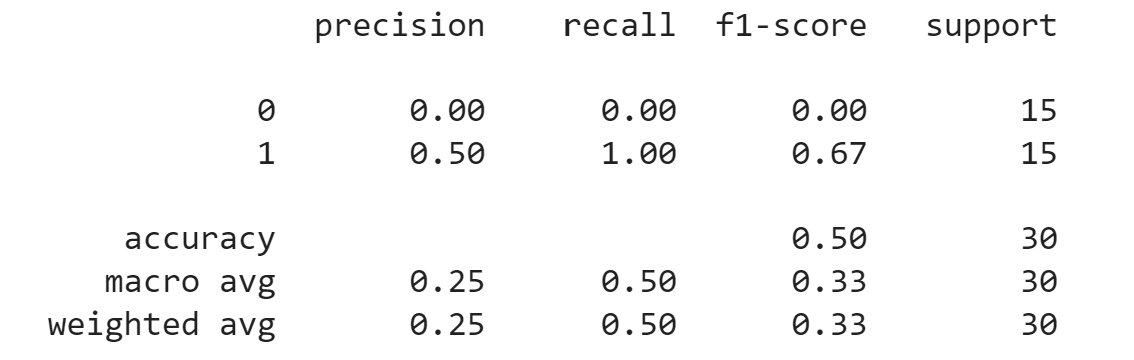
\includegraphics[width=0.75\linewidth]{nn_attempt.png}
    \caption{Basic NN - large dataset}
\end{figure}

With an accuracy of only 0.5 it was clear something went wrong. Although efforts were made to understand why negative sentiment predictions were consistently performing at 0.0 precision, my approach ultimately evolved.

Inspired by the success of the inital logistic regression model, GloVe embedding was utilized in place of one-hot encoding.

\begin{figure}[h]
    \centering
    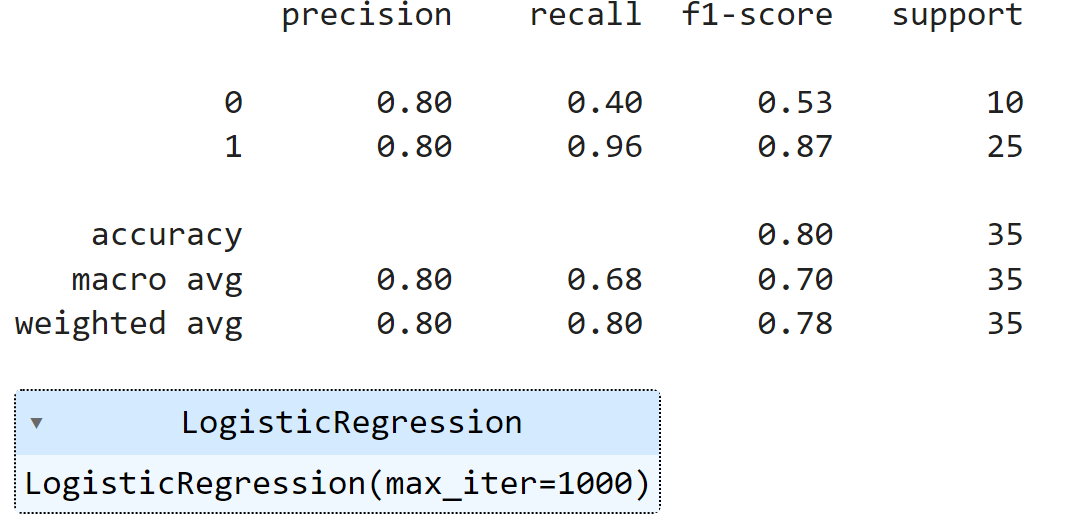
\includegraphics[width=0.75\linewidth]{lr_glove.png}
    \caption{Logistic Regression - GloVe embedding}
\end{figure}


The accuracy was slightly lower than one-hot encoding [0.8 vs 0.86] but did output better word predictions in my opinion. For example, this model was able to identify "creative" and "understanding" as positively associated sentiments. These are on target. 

After this endeavor, an RNN was constructed to actually predict the sentiment of a student course review. 
With a learning rate of 0.1 and 10 epochs, the model was able to achieve an accuracy of 0.762.

\begin{figure}[h]
    \centering
    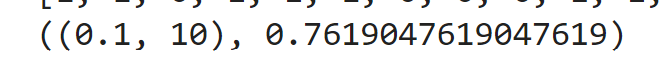
\includegraphics[width=1\linewidth]{rnn_result.png}
    \caption{RNN accuracy \& model parameters}
\end{figure}

As for my POS sidequest, I was able to construct an RNN that predicted tags with high accuracy [0.73 but latex hates my image]. Though it was not the goal, it did give me some confidence moving forward. 

Further attempts were made to integrate GloVe emebedding into this RNN structure. However, due to time constraints, this was not fully completed.

\section{Conclusions}

Through the completion of this project, I was able to show that sentiment classification of student biochemistry class reviews might be possible using the aforementioned methods. Logistic regression consistently performed well on the large dataset. With both one-hot encoding and GloVe embedding, it appears this simple model could be an excellent resource for sentiment analysis.

Furthermore, building an RNN to classify biochemistry reviews showed moderate success. With the execution of Gridsearch and hyperparameter tuning, a final accuracy of 0.762 was achieved. Thus, once can confidently say the model performs better than random chance. With more data, I am optimistic that even better results could be achieved.



\section{Extensions and Future Directions}

With more time and access to larger amounts of data, there are a lot of possibilities for future work.

For example, it would be beneficial to make an easily accessible tool that a professor can enter their reviews into to generate a sentiment prediction. A very loose attempt was made to achieve this goal [using Flask]. In the current scope of this project, the tool might not be very useful, as I did not possess enough data to train the model. Moving forward, I would definitely revisit the possibility of GloVe embedding. Additional hyperparameter tuning would be beneficial as well.

Ultimately, this project serves as a proof of concept. It looks like utilizing a model to process student course reviews might be a beneficial way to quickly return feedback to a STEM [more specifically biochemistry] professor.



\section{Division of Labor}

I completed this experiment entirely by myself, taking on 100\% of the workload



\bibliography{references}
\bibliographystyle{acl_natbib}


\end{document}
